  \documentclass[a4paper]{article}

    \usepackage[english]{babel}
    \usepackage{natbib}
    \usepackage{url}
    \usepackage{longtable}
    \usepackage[utf8x]{inputenc}
    \usepackage{amsmath}
    \usepackage{graphicx}
    \graphicspath{{images/}}
    \usepackage{parskip}
    \usepackage{fancyhdr}
    \usepackage{vmargin}
    \usepackage{blindtext}
    \usepackage[inline]{enumitem}
    \usepackage{usecases}
    \usepackage{tabu}
    \usepackage{float}
    \usepackage{tabularx}   % extensão para tabular
    \usepackage{multirow}
    \usepackage{tabularx}   % extensão para tabular
    \usepackage{multirow}
		
        \addto\captionse{portuguese
      \renewcommand{\contentsname}
        {Índice}
        }
        \setmarginsrb{3 cm}{2.5 cm}{3 cm}{2.5 cm}{1 cm}{1.5 cm}{1 cm}{1.5 cm}
    \title{Autenticação e não repúdio em Arduino} % Title 
    % * <hanifo159@gmail.com> 2016-05-16T17:14:30.866Z:
    %
    % Adicionado Nome do Projeto.
    %
    % ^.
    %\textnormal{}      % Author


    \makeatletter
    \let\thetitle\@title
    \let\theauthor\@author
    \let\thedate\@date
    \makeatother

    \pagestyle{fancy}
    \fancyhf{}
    \rhead{Redes II}
    \lhead{\thetitle}
    \cfoot{\thepage}

    \begin{document}

    %%%%%%%%%%%%%%%%%%%%%%%%%%%%%%%%%%%%%%%%%%%%%%%%%%%%%%%%%%%%%%%%%%%%%%%%%%%%%%%%%%%%%%%%%
    \begin{titlepage}
    \centering
    \vspace*{0.5 cm}
        
\includegraphics[scale = 0.6]{logo_ufc.png}\\[1.0 cm] % University Logo
        \textsc{\Large UNIVERSIDADE FEDERAL DO CEARÁ}\\[0.5 cm] %University
        \textsc{DEPARTAMENTO DE ENGENHARIA DE TELEINFORMÁTICA}\\[1.5 cm]
        \textsc{REDES DE COMPUTADORES II\\ \normalsize TI0155}\\[1.0 cm]  
      \textsc{Prof. Atslands Rego da Rocha}\\[0.5 cm] % Prof Name
      \rule{\linewidth}{0.2 mm} \\[0.4 cm]
    { \huge \bfseries \thetitle}\\
    %
\includegraphics[scale = 0.6]{Template/2.jpg}\\
    \rule{\linewidth}{0.2 mm} \\[0.5 cm]
    \begin{minipage}{0.4\textwidth}
    \begin{flushleft} \large
    \emph{Equipe:}\\
    \textnormal{Bruno Augusto\\Liuz Guerreiro\\Luan Pinheiro\\Matheus Costa\\Paulo César\\Reginaldo da Silva}
    \end{flushleft}
    \end{minipage}~
    \begin{minipage}{0.4\textwidth}
    \begin{flushright} \large
    \emph{Matrícula:} \\
          394185\\371986\\371990\\371846\\372015\\371860                 % Your Student Number
          \end{flushright}
          \end{minipage}\\[2 cm]
          
          {\large \today}\\[2 cm]
          
          \vfill
          
          \end{titlepage}
                      %Fim da Capa
    %%%%%%%%%%%%%%%%%%%%%%%%%%%%%%%%%%%%%%%%%%%%%%%%%%%%%%%%%%%%%%%%%%%%%%%%%%%%%%%%%%%%%%%%%

    \tableofcontents
    \thispagestyle{empty}
    \pagebreak

    %%%%%%%%%%%%%%%%%%%%%%%%%%%%%%%%%%%%%%%%%%%%%%%%%%%%%%%%%%%%%%%%%%%%%%%%%%%%%%%%%%%%%%%%%
    \section{Introdução}
    \subsection{Área de Configuração}
    \paragraph{}
    	A área de gerenciamento de configuração do modelo FCAPS está focada no monitoramento de informações sobre as configurações do sistema, ou qualquer mudança que possa ocorrer. A importância dessa área está em evitar problemas que possam ocorrer na rede, uma vez que muitos destes estão diretamente ligados à alterações nos arquivos de configurações, atualizações de software ou mudanças no hardware. 
    
    \subsection{Objetivos da Área}
    \paragraph{}
    Os objetivos do gerenciamento de configuração incluem:
    \begin{itemize}
	\item Recolher e armazenar as configurações de dispositivos de rede;
    \item Controlar as alterações que são feitas;
	\item Simplificar a configuração dos dispositivos;
    \item Manter atualizado o inventario de equipamentos e programas da rede.  
	\end{itemize}
  
  \newpage 
   \section{Objetos da MIB}
   \paragraph{}
   Nesta seção estão apresentando os os objetos mais relevantes para a área de configuração na rede em estudo, assim como quais informações importantes podem ser extraídas deles.
     
     %%%%%%%%%%%%%%%%%%%%%%%%%%%% INICIO TABELA DE OBJETOS &&&&&&&&&&&&&&&&&&&&
   \begin{table}[H]
    \begin{tabu} to \linewidth {>{\bfseries}X[0.6]|X[3l]|X[2l]}
    \everyrow{\tabucline[.2pt]-}
    \rowfont\bfseries
    Objeto  & Descrição & Informações \\  \hline
    
    \texttt{Obj.1}  & Descrição textual do dispositivo. Contendo o nome completo,  identificador, informações dos hardware, sistema operacional e comunicação com a rede. & obtido através do OCs essas informações são relevantes para um melhor entendimento geral sobre a máquina que está sendo analisada.\\ 
    \texttt{Obj.2}  & Tempo em que o subsistema de gerência de rede da entidade foi reinicializado. Havendo uma trap sempre que for reinicializado. & essa informação é útil para podermos perceber o tempo que a gerência está em execução e ver a ocorrência de algum problema que tirou alguma das máquinas do ar.\\ 
    \texttt{Obj.3}  & Informações de nome do nodo. Dado administrativamente.
 & obtido através do Ntop, essa informação é útil para o caso de termos uma rede subdividida, através desse objeto podemos identificar cada uma das subdivisões da rede .\\ 
    \texttt{Obj.4}  & Informações do responsável por esse nodo, nome e como entrar em contato. &obtido através do Ntop, essa informação é relevante para identificar o administrador da rede em questão, no caso de uma rede dividida em sub redes podemos identificar o administrador de cada uma delas. \\ 
  
    \end{tabu}
    \end{table}
  
   %%%%%%%%%%%%%%%%%%%%%%%%%%%% FIM TABELA DE OBJETOS &&&&&&&&&&&&&&&&&&&&
   %%%%%%%%%%%%%%%%%%%%%%%%%%%% INICIO TABELA DE OBJETOS &&&&&&&&&&&&&&&&&&&&
   \begin{table}[H]
    \begin{tabu} to \linewidth {>{\bfseries}X[0.6]|X[3l]|X[2l]}
    \everyrow{\tabucline[.2pt]-}
    \rowfont\bfseries
    Objeto  & Descrição & Informações \\  \hline
    
   \texttt{Obj.5}  & Localização física do dispositivo.
 & obtido através do Ntop, essas informações são relevantes para poder identificar a localização da máquina que está sendo analisada. neste caso não é de extrema relevância uma vez que a localização da rede é conhecida . \\ 
 	 \texttt{Obj.6}  &Serviços suportados pelo dispositivo;
 & obtido através do Ntop, essas informações são relevantes para podermos analisar quais serviços estão disponíveis na rede como por exemplo http, mail-pop e mail-SMTP. \\ 
 	\texttt{Obj.7}  &Tabela contendo o endereço IP do dispositivo.
 & obtido através do Ntop, essas informações são relevantes para poder identificar a máquina que está sendo analisada e poder localizá-la na internet . \\
 	\texttt{Obj.8}  & Tabela de interfaces com o dispositivos:
    \begin{itemize}
	\item Nome do produto, versão do hardware;
    \item Tamanho do maior datagrama que pode ser enviado ou recebido pela rede;
    \item Estimativa de velocidade;
    \item Estado da interface.
\end{itemize}
 & obtido através do Ntop, essas informações são relevantes para ter uma visão acerca dos  aspectos de conexão podendo informar a necessidade de aprimoramentos nos enlaces e/ou nas máquinas.\\
 \texttt{Obj.9}  &Tabela contendo endereços IP:
    \begin{itemize}
	\item Endereço IP;
    \item Máscara da sub-rede.
\end{itemize}
 &  obtido através do Ntop, essas informações são relevantes para ter uma visão mais geral sobre as conexões da rede em si e de como a rede está estruturada. \\ 
   
    \end{tabu}
    \end{table}
  
   %%%%%%%%%%%%%%%%%%%%%%%%%%%% FIM TABELA DE OBJETOS &&&&&&&&&&&&&&&&&&&&
  
  \section{Análise da rede e Resultados}
  	 
  
  \subsection{A rede em análise}
  \paragraph{}
    A rede em análise consiste em uma lan house com 6 máquinas com o sistema operacional windows e com configuração semelhante , um notebook com sistema operacional linux  e outros dispositivos não gerenciados como celulares e impressoras.
  \paragraph{}
     Devido a funcionalidade específica da rede em questão deve-se prezar por qualidade de conexão e por uma configuração mediana nas máquinas, não sendo necessário grande poder de processamento ou muito espaço de armazenamento disponível.
  \paragraph{}
    Em nível de softwares , temos a necessidade de um bom antivírus uma vez que a máquina é utilizada por diversos usuários. assim como os programas mais utilizados como jogos, editores de texto e navegadores web.
    
  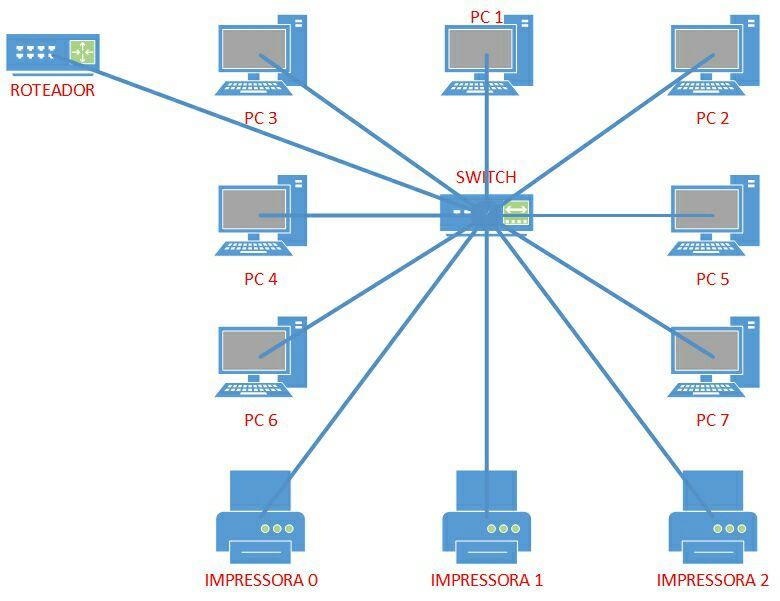
\includegraphics[scale = 0.55]{topologia.jpg}\\

    \subsection{Inventário}
     É importante fazer um inventário para se ter um conhecimento detalhado da rede e poder controlar a localização e a utilização dos equipamentos da rede. Com o inventário a manutenção e reposição de dispositivos de rede ficam mais fáceis e é possível ter um melhor monitoramento dos mesmos.
	 \paragraph{}
	O inventário de dispositivos (hardware e software) da rede serve para coletar os dados relevantes sobre todos os dispositivos da rede,  nome da máquina, usuário, processador, memória, HD, placa mãe, versão do antivírus, versão do sistema operacional, endereçamento IP e MAC são interessantes de ser levantados e estatísticas detalhadas.
	\paragraph{}
    Para realizar o inventário da rede utilizamos o software OCS Inventory v2.0.2. O software é livre e permite aos usurários inventariar ativos de TI na rede. O OCS coleta informações sobre o hardware e o software das máquinas em rede executando um programa cliente do OCS ("OCS Inventory Agent"). O OSC pode visualizar o inventário por meio de uma interface web.\\
    \begin{center}
     
\includegraphics[scale = 0.9]{ocs.png}\\
     A instação do software foi feita no Ubuntu 12, utilizando o tutorial disponivel no endereço: www.vivaolinux.om.br/Instalando-o-OCS-Inventory
    \end{center}
  	\subsubsection{Activity}
    \paragraph{}
    Na aba \texttt{Activity} podemos visualizar a quantidade de máquinas da rede, máquinas que estão visiveis, máquinas acessadas pelo servidor e número de máquinas que fizeram o inventário.\\
   
   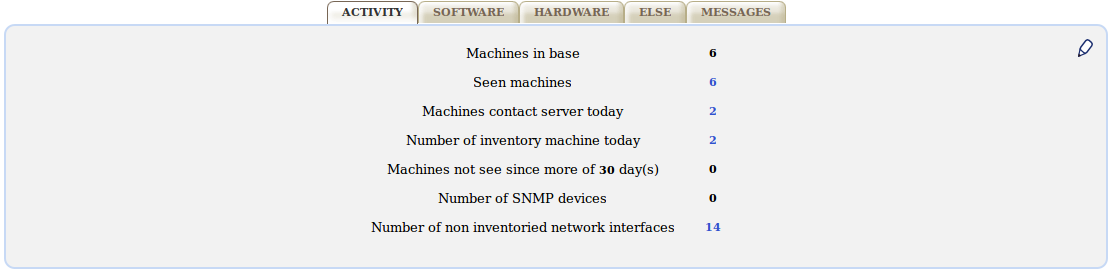
\includegraphics[scale = 0.3]{activity.png}\\
   
   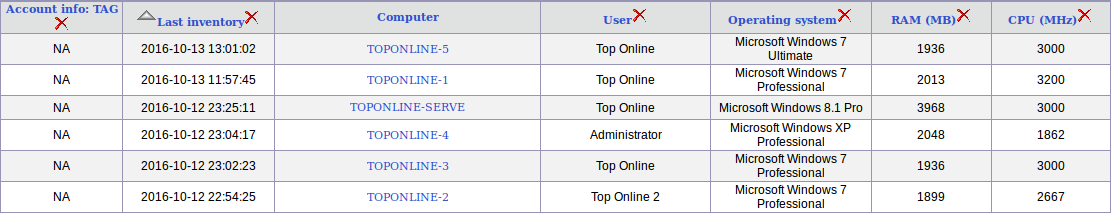
\includegraphics[scale = 0.3]{maquinas.png}\\
 	\paragraph{}
 	Nesta aba podemos perceber que na rede realmente existem 6 máquinas e que todas as 6 estão visíveis para o gerente, podemos também perceber um elevado número de dispositivos não gerenciados , o que pode vir a ser uma falha na gerência, esse alto número de dispositivos visíveis e não gerenciáveis se dá pelo uso doméstico da rede pelos donos da lan house, no aspecto de rede estes dispositivos estão sendo gerenciados pelo Ntop.
    \subsubsection{Software}
    \paragraph{}
     Na aba \texttt{Software} podemos visualizar os diferentes sistemas operacionais e os diferentes agentes instalados nos dispositivos da rede.
    
    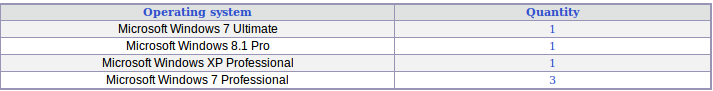
\includegraphics[scale = 0.5]{so.png}\\
    \paragraph{}
    Nesta aba podemos perceber a presença de 4 sistemas operacionais diferentes, entretanto ao clicar sobre esse dados percebemos que todos são Windows , sendo apenas versões diferentes. Tendo em vista que as máquinas possuem finalidades similares seria uma boa prática manter a mesma versão do sistema operacional para facilitar o gerenciamento dos softwares a serem instalados, uma vez que podem diferir entre as versões do SO.   
    \subsubsection{Hardware}
     \paragraph{}
  Na aba \texttt{Hardware} vemos os componentes que fazem parte dos dispositivos da rede, principalmente os processadores e a resoluções. 
  	
    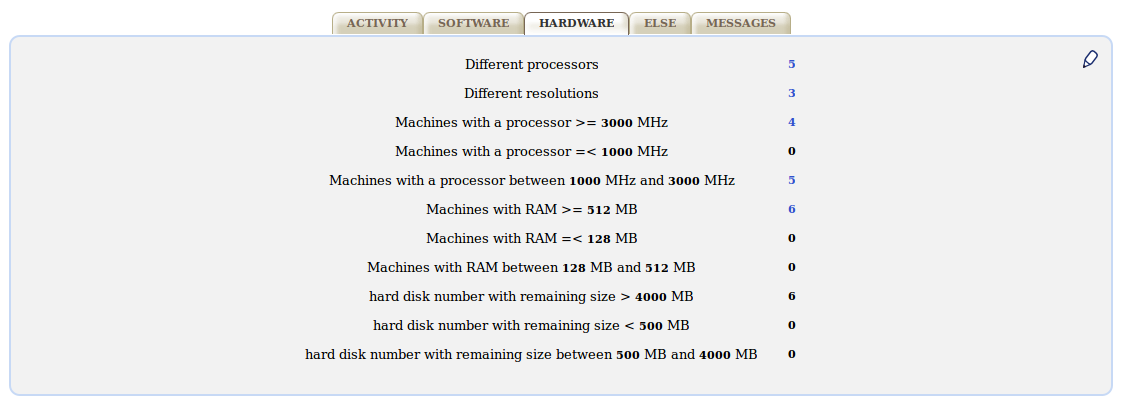
\includegraphics[scale = 0.3]{hardware.png}\\
  	
    Abaixo segue os processadores das máquinas.
    
    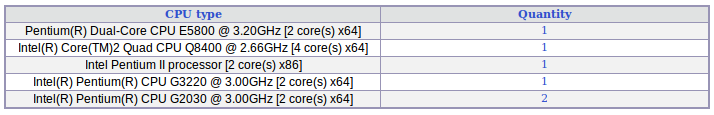
\includegraphics[scale = 0.5]{processors.png}\\
    \paragraph{}
    Nesta aba podemos analisar as diferentes especificações de hardware, a partir destas informações podemos perceber que as configurações em nível de hardware das máquinas são bem parecidas, analisando os processadores podemos perceber que apenas uma das máquinas possui mais de 2 núcleos de processamento, esta máquina com maior potência computacional é a responsável pela gerência da lan house.
     \paragraph{}
    Analisando as resoluções percebemos que são as mesmas com exceção da máquina da gerência. Através dessas informações podemos traçar o perfil da rede , com 5 máquinas padrão para os usuários e uma máquina para a gerência da lan house
    \subsubsection{Else}
    \paragraph{}
    Na barra \texttt{Else} encontra-se os o número de diferentes Workgroup, diferentes TAG, diferentes IPSUBNET, máquinas com implementação de software pendente e máquinas que possuem algum pacote com erro.
    
        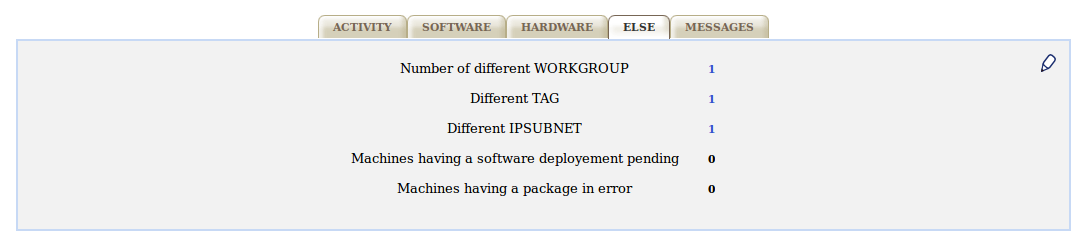
\includegraphics[scale = 0.3]{else.png}\\
	\paragraph{}
   	 Nesta aba podemos perceber ausência de pacotes em erro, o que é um bom indicador.
	\subsubsection{Visualizando informações no OCS}
    \paragraph{}
	Selecionamos uma máquina qualquer para demostrar quais informações podemos visualizar através da interface web do OCS, todas as operações realizadas também se aplicam nas outras máquinas da rede.
    
	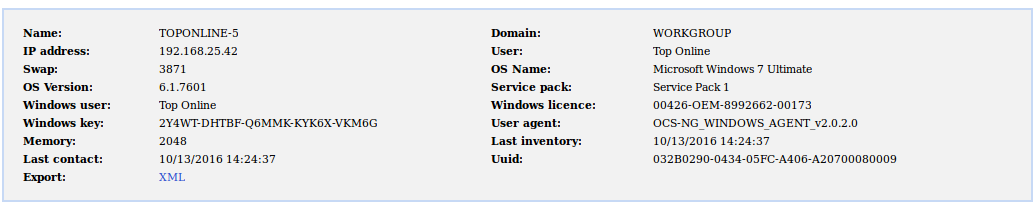
\includegraphics[scale = 0.48]{machine.png}\\
    
  \paragraph{} Os ícones representam os objetos dos dispositivos (processador, memória, storage, discos, placa de vídeo, placa de som, redes, controladores, slots, portas etc.) e ao serem selecionados o OCS mostra suas especificações. A figura abaixo ilustra os ícones presentes no OCS. A inteface é intuitiva e basta selecionar um dos ícones para obter as informações.
  
  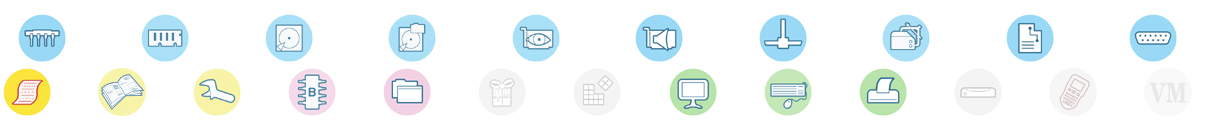
\includegraphics[scale = 0.39]{icones.png}\\
  
  Iremos visulizar algumas especificações da máquina em questão.
  \begin{itemize}
  \item Processador 
\includegraphics[scale = 1.8]{pro.png}\\
  
  	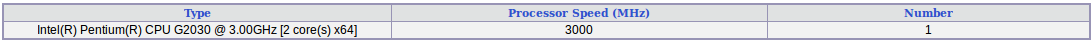
\includegraphics[scale = 0.4]{process.png}
    \paragraph{}
    Podemos perceber que o processador utilizado na máquina não é um de alta potência entretanto, se alinha com o uso médio em uma lan house
    
  \item Memória 
\includegraphics[scale = 0.5]{memory.png}\\
  
  	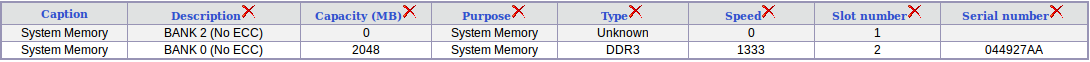
\includegraphics[scale = 0.4]{memoria.png}
	\paragraph{}
    Na análise da memória podemos perceber que a placa mãe possui dois slots para memória mas apenas um está ocupado , o que poderia vir a ser um problema, entretanto a memória DDR3 que utilizada prove 2 Giga para a máquina , sendo um valor suficiente para o uso comum.
\item Storage 
\includegraphics[scale = 0.5]{stor.png}\\
  
  	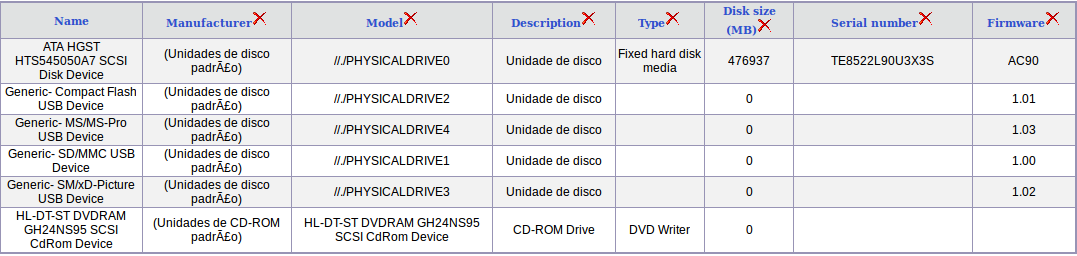
\includegraphics[scale = 0.4]{storage.png}
  	\paragraph{}
    Assim como já foi previamente analisado não há uma forte necessidade por grande espaço de armazenamento, uma vez que o uso de uma máquina em uma lan house não consiste em guardar informações na máquina. Logo o disco rígido com 500 giga é mais que suficiente para esta máquina.
 \item Discos 
\includegraphics[scale = 0.5]{disk.png}\\
  
  	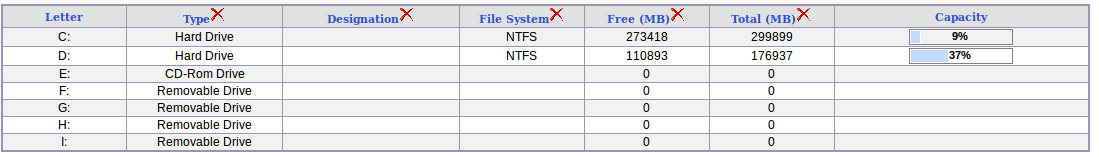
\includegraphics[scale = 0.4]{discos.png}
    \paragraph{}
    \textnormal{Análise dos discos apenas corrobora a análise do storage ao mostrar que nenhuma das partições possui mais que 40 \% ocupados. }   
  \item Placa de Vídeo 
\includegraphics[scale = 0.5]{card.png}\\
  
  	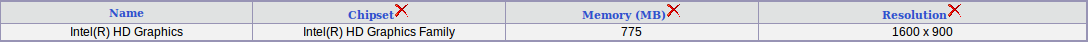
\includegraphics[scale = 0.4]{video.png}
    \paragraph{}
    A placa de vídeo utilizada na máquina é o chipset da intel, não possuindo assim grande poder gráfico, entretanto condiz com uso da lan house que consiste em navegação web e jogos de baixo aporte gráfico como C.S 1.6 e Combat Arms.
   \item Placa de Som 
\includegraphics[scale = 1.8]{sound.png}\\
  
  	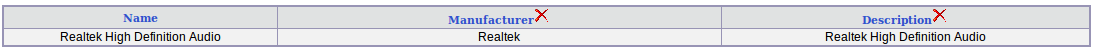
\includegraphics[scale = 0.4]{somm.png}
     \paragraph{}
     As interface de áudio é uma realtek básica , condizente com o uso na lan house.
    \item Interfaces de Rede 
\includegraphics[scale = 1.8]{network.png}\\
  
  	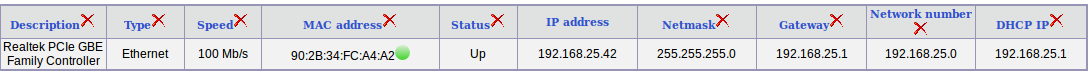
\includegraphics[scale = 0.4]{rede.png}
    \paragraph{}
    A interface de rede presente na máquina indica a opção por internet cabeada o que é uma decisão acertada pois garante menor perda de pacote e maior estabilidade na conexão. também podemos perceber que a velocidade de 100 Mb/s é satisfatória para o uso de navegação web.
    \item Controladores 
\includegraphics[scale = 0.5]{controllers.png}\\
  
  	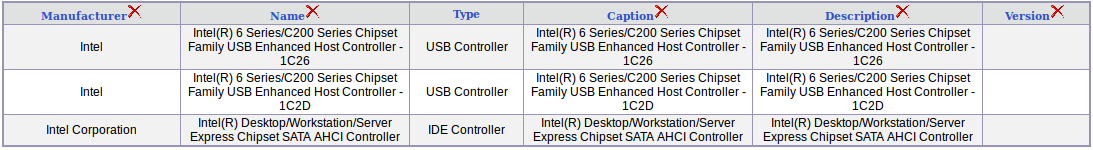
\includegraphics[scale = 0.4]{controlador.png}
    
    \item Slots 
\includegraphics[scale = 1.8]{slots.png}\\
  
  	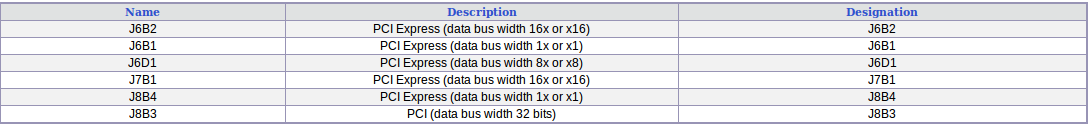
\includegraphics[scale = 0.4]{slot.png}
    
    \item Portas 
\includegraphics[scale = 1.8]{ports.png}\\
  
  	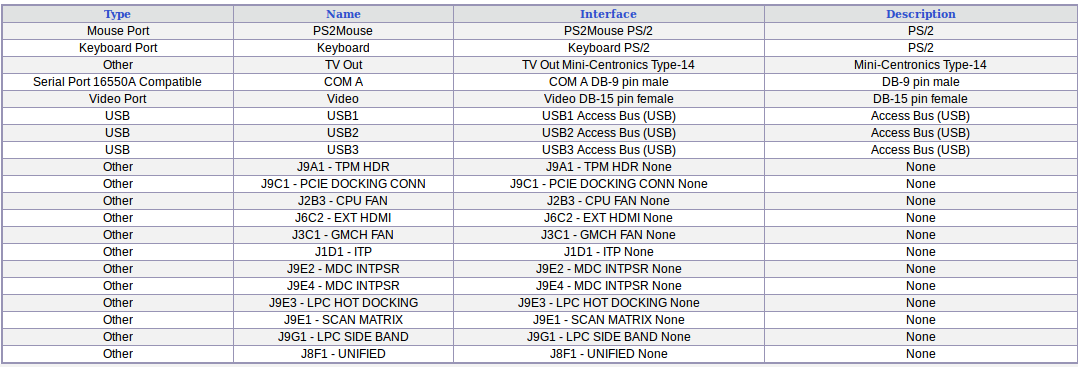
\includegraphics[scale = 0.4]{portas.png}
    
    \item Bios 
\includegraphics[scale = 0.5]{bios.png}\\
  
  	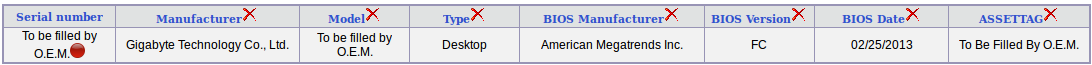
\includegraphics[scale = 0.4]{bioo.png}
    
    \item Software 
\includegraphics[scale = 1.8]{software.png}\\
  
  	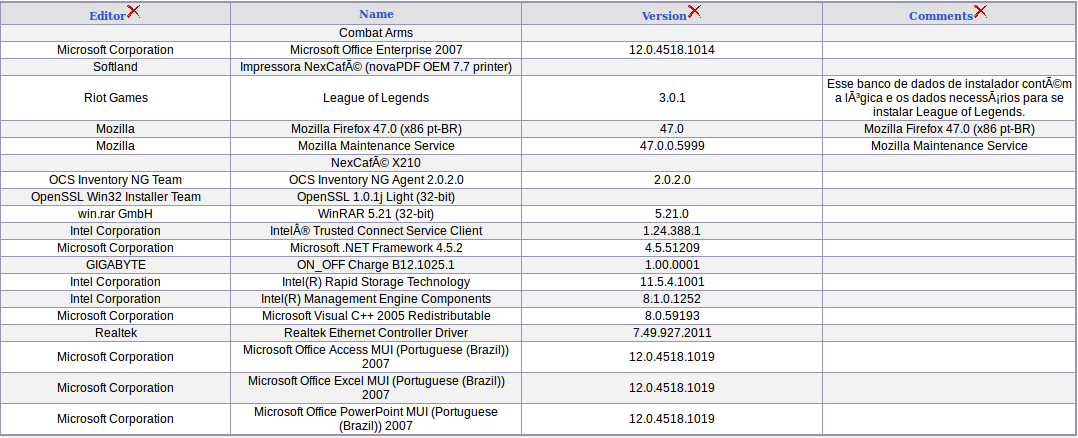
\includegraphics[scale = 0.4]{soft.png}
    \paragraph{}
    Quanto aos softwares podemos constatar que são basicamente os jogos, pacote office e navegadores web, outros programas também estão instalados totalizando 243 softwares. outro ponto a se destacar é a presença de um antivírus.
    
    \item Monitor 
\includegraphics[scale = 1.8]{monitor.png}\\
  
  
  	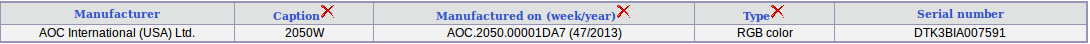
\includegraphics[scale = 0.4]{monitore.png}
    
    \item Input Devices 
\includegraphics[scale = 0.45]{input.png}\\
  
  	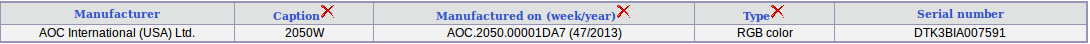
\includegraphics[scale = 0.4]{monitore.png}
    
    \item Impressoras 
\includegraphics[scale = 1.8]{printer.png}\\
  
  	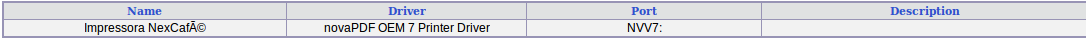
\includegraphics[scale = 0.4]{impress.png}
 
 \end{itemize}
 
 \subsection{Análise da rede}
 \paragraph{}
 A rede local em análise 192.168.25.0  foi monitorada usando a ferramenta ntopng v2.4.160627. 
Na figura abaixo vemos os hosts ativos na rede e suas informações como tráfego total e taxa de transferência.

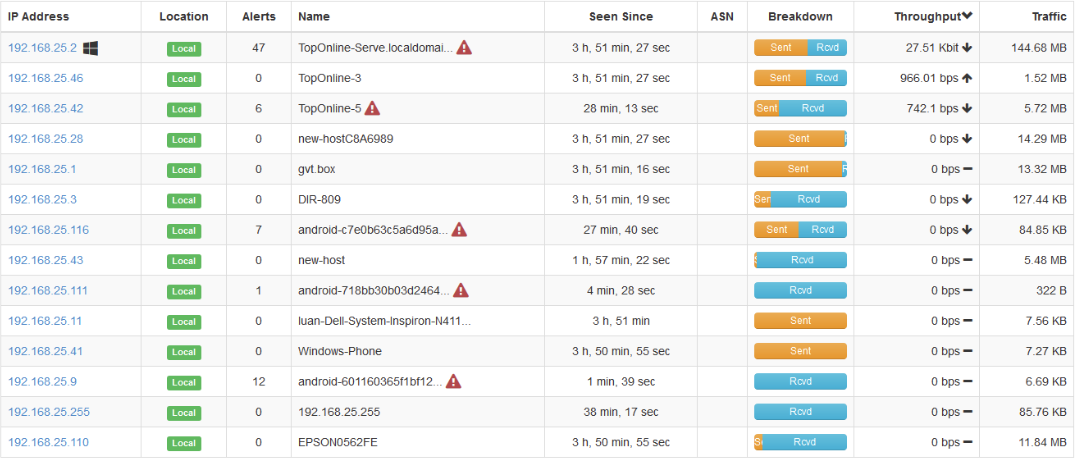
\includegraphics[scale = 0.4]{ntop11.png}

\paragraph{}A rede apresenta um servidor, que é identificado pelo nome do Host e também pela quantidade de dados trafegados. Informações mais detalhadas são obtidas acessando o host sob análise. Verifica-se também o gateway da rede que como é esperado apresenta maior envio de dados do que recepção. Abaixo algumas informações de tráfego da rede.


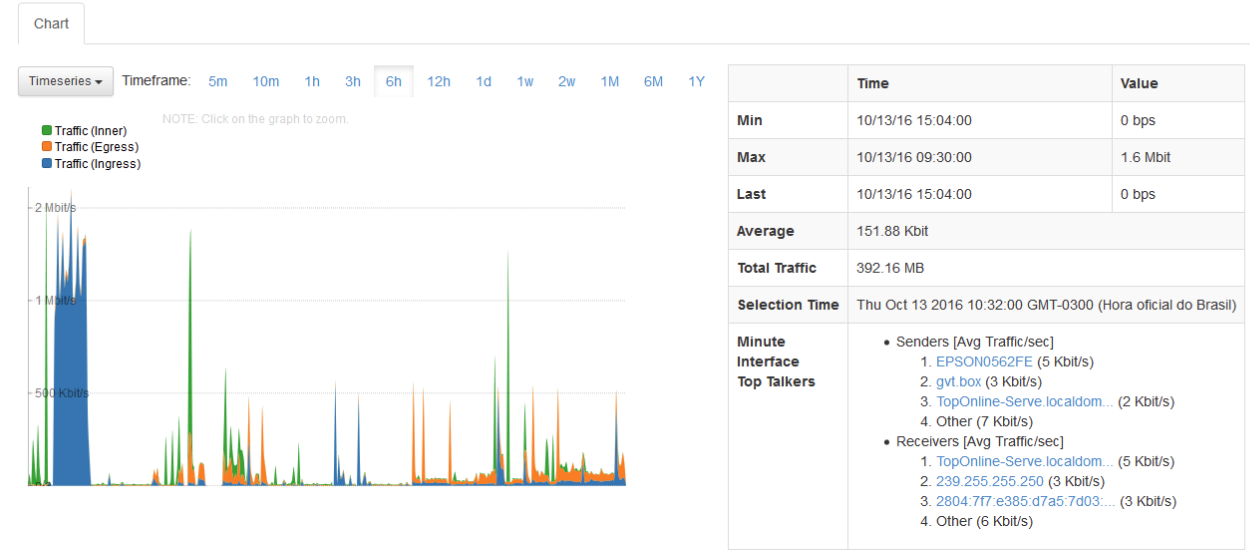
\includegraphics[scale = 0.35]{ntop2.png}

\paragraph{}Uma análise mais profunda pode apresentar a necessidade de alterar configurações da rede, por exemplo fechar portas que possam estar sendo utilizadas para gerar um tráfego de dados muito alto. Também é possível bloquear o acesso a determinados serviços ou analisar o seu uso ao longo do tempo. Como exemplo a figura abaixo mostra percentualmente o uso de aplicações na rede.

 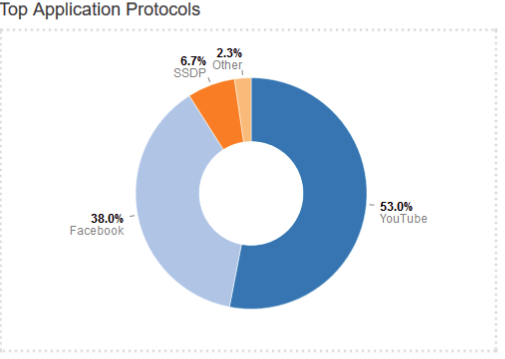
\includegraphics[scale = 0.35]{ntop3.png}
    
 Portas mais usadas:
 
  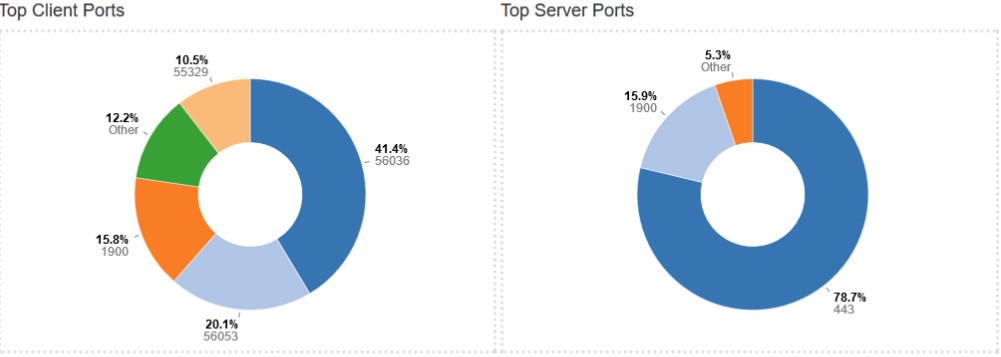
\includegraphics[scale = 0.35]{ntop4.png}
    
   \paragraph{} Abaixo vemos os hosts que apresentam maior tráfego. Se um desses hosts estiver gerando um tráfego fora dos padrões uma alteração nas configurações pode diminuir este tráfego ou encaminhá-lo para outro roteador.
    
    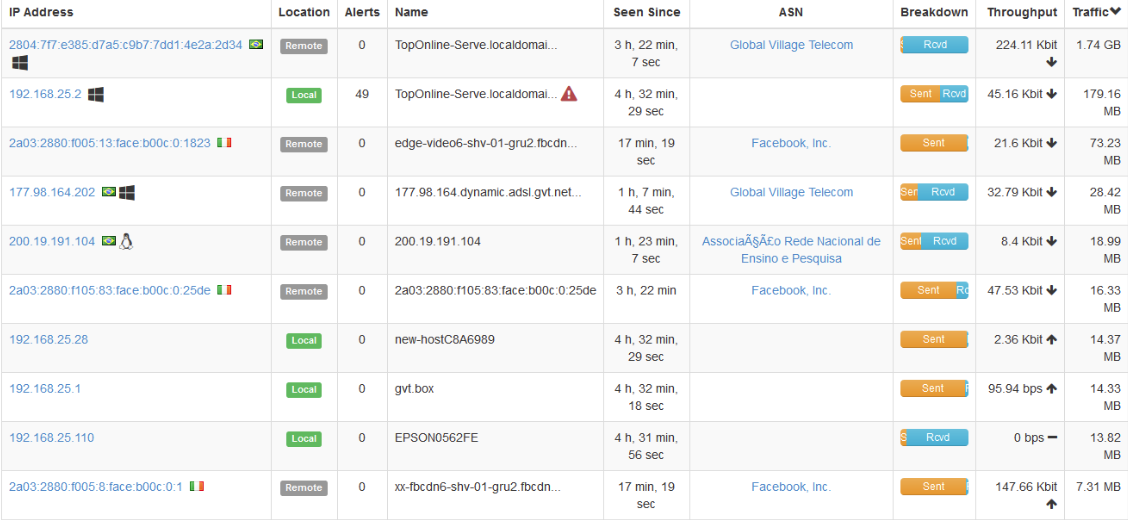
\includegraphics[scale = 0.35]{ntop5.png}
    
   \paragraph{} A ferramenta ntopng oferece uma gama grande de funcionalidades que podem ser usadas para a configuração e monitoramento da rede.
    
    \section{Conclusões}
  \paragraph{}
  Neste relatório apresentamos os motivos da necessidade de fornecer ferramentas adequadas ao administrador, ou responsável pela configuração.
  
\paragraph{}O gerenciamento de configuração permite que a equipe como administrador de rede saiba quais os dispositivos fazem parte da rede e quais são as suas configurações de hardware e software. Dessa forma é possível analisar, consultar, configurar, monitorar os nodos da rede.

\paragraph{}A arquitetura do sistema tem 5 elementos fundamentais, são eles: um gerenciador de rede, um conjunto de dispositivos gerenciados remotamente, as bases de informações de gerenciamento(MIB), os agentes remotos, um protocolo para comunicação entre gerenciador de rede e os dispositivos remotos.
\paragraph{}A escolha da rede foi um exemplo pequeno, porém válido para demonstrar que redes de grande ou médio porte precisam ter sua configuração monitorada.

\paragraph{}Através dos dados obtidos pela gerência de configuração, o administrador da rede pode analisar e projetar uma possível expansão ou mudanças nos parâmetros dos dispositivos da rede.  No nosso caso, visualizamos o perfil de usuários da lan house, analisamos quais são os serviços e aplicações mais utilizadas, o fluxo da rede dentre outras coisas, e chegamos a conclusão que a atual configuração das máquinas atende de maneira satisfatória a maioria das tarefas realizadas pelos usuários. Uma mudança ou atualização dos componentes deve ser feita a médio ou longo prazo. 
    
    \end{document}
    